\documentclass[12pt]{article}
\usepackage{pgfplots}
\newcommand{\piRsquare}{\pi r^2}

\title{Sample \LaTeX{} Document}			
\author{Masiar Babazadeh}	
\date{\today}

\begin{document}
\maketitle

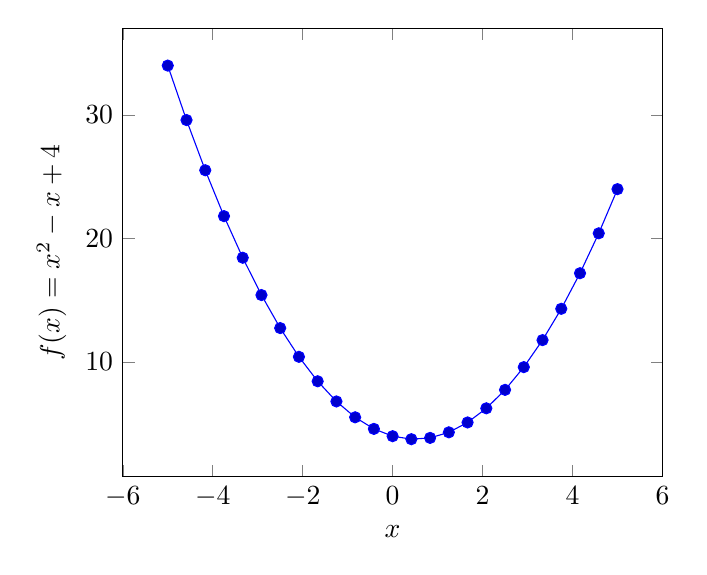
\begin{tikzpicture}
	\begin{axis}[
		xlabel=$x$,
		ylabel={$f(x) = x^2 - x +4$}
	]
	% use TeX as calculator:
	\addplot {x^2 - x +4};
	\end{axis}
\end{tikzpicture}

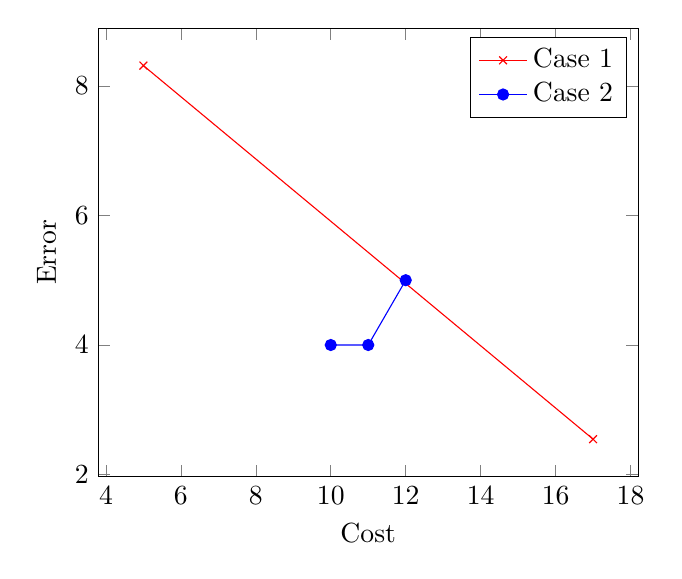
\begin{tikzpicture}
\begin{axis}[
	xlabel=Cost,
	ylabel=Error]
\addplot[color=red,mark=x] coordinates {
	(5,    8.31160034)
	(17,   2.54685)
};

\addplot[color=blue,mark=*] coordinates {
		(10, 4)
		(11, 4)
		(12, 5)
};

\legend{Case 1,Case 2}
\end{axis}
\end{tikzpicture}


\end{document}             % End of document.